\documentclass{beamer}
  \usepackage{ctex}
  \usepackage{beamerthemesplit}
  %\usepackage{beamerthemeshadow}
  %\usepackage[width=2cm]{beamerthemesidebar}
  \usepackage{amsmath, amssymb}
  \usepackage{graphicx}
  \usepackage{epigraph}

  % 标题、作者、日期信息
  \title{\LaTeX 入门介绍}
  \author{桂义林}
  \date{2014年11月9日}

  % 在每一个Section之前显示目录
  \AtBeginSection[]
  {
    \begin{frame}[shrink]
      \frametitle{目录}
      \tableofcontents[current, currentsubsection]
    \end{frame}
  }

  % 在每一个Subsection之前显示目录
  \AtBeginSubsection[]
  {
    \begin{frame}[shrink]
      \frametitle{目录}
      \tableofcontents[current, currentsubsection]
    \end{frame}
  }

  %%%%%%%%%%%%%%%%%%%%%%%%%%%%%%%%%%%%%%%%%%%%%%%%%%%%%%%%%%%%%
  % 文档开始
  \begin{document}

  % 生成标题页
  \frame{\titlepage}

  % 生成提纲页
  \section*{提纲}
  \frame
  {
    \frametitle{\secname}
    \tableofcontents[hideallsubsections]  % 自动生成目录
  }

  %%%%%%%%%%%%%%%%%%%%%%%%%%%%%%%%%%%%%%%%%%%%%%%%%
  % Section 1. TeX/LaTeX概览                      %
  %%%%%%%%%%%%%%%%%%%%%%%%%%%%%%%%%%%%%%%%%%%%%%%%%
  \section{\TeX /\LaTeX 概述}

  % 1.1 什么是TeX
  \subsection{什么是\TeX}
  \frame
  {
    \frametitle{\subsecname}
    \begin{itemize}
    \item 高纳德,TAOCP的作者
      \begin{figure}
      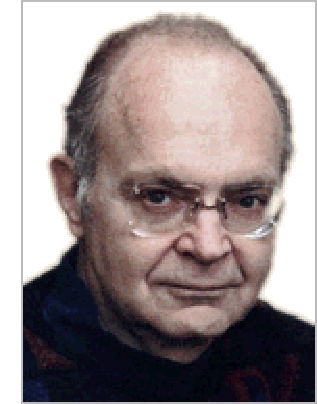
\includegraphics[scale=0.4]{Knuth.pdf}
      \end{figure}
    \item \TeX 是由著名的计算机科学家Donald E. Knuth发明的电子排版系统
    \item \TeX 排版生成高质量的DVI(DeVice Independent)文件,几乎可以在所有的输出设备上输出
    \end{itemize}
  }

  \frame
  {
    \frametitle{\subsecname}
    \begin{itemize}
    \item \TeX 是学术界内公认的标准,一些顶级期刊、会议只接受\TeX 排版的论文投稿
    \item \TeX 是免费的,Knuth公开了所有源代码
    \item \TeX 版本号:3.14159265 $\rightarrow \pi$
    \end{itemize}
  }

  % 1.2 什么是LaTeX
  \subsection{什么是\LaTeX}
  \frame
  {
    \frametitle{\subsecname}
    \begin{itemize}
    \item \TeX 提供了功能强大的排版语言,900多条指令,用户可通过宏进行功能扩展
    \item Knuth设计了一个名为Plain TeX的基本宏集,以与低层次的TeX呼应。该宏集的重点还仅仅在于如何排版的角度,而非从作者的角度出发,使用它需要较多编程技巧
    \item \LaTeX 由Leslie Lamport开发,是目前最流行的TeX宏集,它提供了一组生成复杂文档所需的高级命令,使用者没有较深入的排版和编程知识也可以充分利用TeX的强大功能,可以在短时间内生成具有印刷品级质量的文档。对于生成复杂表格和数学公式,LaTeX的表现尤为出色
    \end{itemize}
  }

  \frame
  {
    \frametitle{\TeX \LaTeX 如何发音}
    \begin{itemize}
    \item \TeX 的名字来自于大写的希腊字母(tau, epsilon, chi)组成。在希腊语中这个词的意思是“科技”和“艺术”
    \item \TeX 读作"tech",\LaTeX 读作"lei tech"
    \item latex(|lateks|)在英文中是“橡胶浆”的意思
    \end{itemize}
  }

  \frame
  {
    \frametitle{TeX Users Group}
    \begin{figure}
    
\includegraphics[scale=0.5]{TUGlog.pdf}
    \end{figure}
    在TeX出生两岁时,第一个TeX用户组织于1980年2月22日在斯坦福大学成立,简称TUG。它是由对排版技术和字体设计感兴趣的TeX系统用户自发组成的社团,其宗旨是促进和扩展TeX系统的应用、维护TeX系统的完整性和可移植性、支持高质量电子文稿制作的改革与创新。
  }

  \frame
  {
    \frametitle{\TeX 软件套装(发行版)}
    \begin{description}
    \item[TeXLive]
      TUG官方的发行版,各大平台通吃。TeXLive2014
    \item[MikTeX]
      Windows平台下用户最多的发行版
    \item[MacTeX]
      Mac OS X上的版本
    \item[CTeX]
      国内流行的MikTeX衍生版本,www.ctex.org
    \end{description}
  }

  %%%%%%%%%%%%%%%%%%%%%%%%%%%%%%%%%%%%%%%%%%%%%%%%%%%%%%%%%%%%%

  %%%%%%%%%%%%%%%%%%%%%%%%%%%%%%%%%%%%%%%%%%%%%%%%%
  % Section 2. 为什么要使用LaTeX                  %
  %%%%%%%%%%%%%%%%%%%%%%%%%%%%%%%%%%%%%%%%%%%%%%%%%
  \section{为什么要使用\LaTeX}

  % 2.1 LaTeX的优点
  \subsection{\LaTeX 的优势}
  \frame
  {
    \frametitle{\subsecname}
    \begin{description}
    \item[高质量的输出]
      专业级的排版系统,稳定、美观、质量高
    \item[简单而又灵活]
      通过文本文件保存,熟悉后直接阅读源码也能看懂大部分内容。除了排版文字,还可以排版乐谱、象棋棋谱等
    \item[可编程]
      使用代码控制章节、图表、参考文献等,精确
    \item[超级技术支持]
      \TeX 并不是由某个公司垄断开发的,所以世界各地的使用者采用统一的技术支持方式:E-mail, WWW, FTP。免费,分享
    \end{description}
  }

  % 2.2 LaTeX的劣势
  \subsection{\LaTeX 的劣势}
  \frame
  {
    \frametitle{\subsecname}
    \begin{description}
    \item[学习曲线]
      上手易,精通难
    \item[易用性]
      在处理对格式要求不严格的文档时,可能还是Word好用
    \item[可见性]
      \LaTeX 非所见即所得(WYSIWYG),需要经过编译生成可见文档
    \end{description}
  }

  % LaTeX与Word的比较
  \frame
  {
    \frametitle{\LaTeX 与 Word 的比较}
    \begin{itemize}
    \item[*] Word简单易用,针对可视编辑,所见即所得
    \item[*] 适合普通办公文档编辑
    \end{itemize}

    \begin{itemize}
    \item \LaTeX 稳定,针对文章逻辑结构,所想即所得(WYTIWYG)
    \item 生成的文档质量比Word高
    \item 数学公式编辑能力很强
    \item 适合科技论文书籍的排版
    \end{itemize}
  }

  %%%%%%%%%%%%%%%%%%%%%%%%%%%%%%%%%%%%%%%%%%%%%%%%%%%%%%%%%%%%%

  %%%%%%%%%%%%%%%%%%%%%%%%%%%%%%%%%%%%%%%%%%%%%%%%%
  % Section 3. LaTeX文档制作入门
  %%%%%%%%%%%%%%%%%%%%%%%%%%%%%%%%%%%%%%%%%%%%%%%%%

  \section{\LaTeX 文档制作入门}

  % 3.1 基本排版命令
  \subsection{\LaTeX 排版命令}
  \frame
  {
    \frametitle{\subsecname}
    \TeX 系统是根据命令(预定义宏/函数)编译文档的,\LaTeX 的命令一般有如下形式\\
    \begin{center}
    $\backslash$command[options]{argument}
    \end{center}

    典型的文档头声明示例\\
    $\backslash$documentclass\{article\}\\
    $\backslash$usepackage\{graphicx\}\\
    $\backslash$title\{Test\}\\
    $\backslash$author\{Test\}\\
    $\backslash$date\{$\backslash$today\}
  }

  \frame
  {
    \frametitle{\LaTeX 文档结构}
    \begin{itemize}
    \item \LaTeX 预制了几种不同类型的文档
      \begin{itemize}
      \item[-] article: 一般的期刊文章
      \item[-] book: 书
      \item[-] report: 研究报告
      \end{itemize}
    \item CTeX宏包定义了一些中文文档类
      \begin{itemize}
      \item[-] ctexart
      \item[-] ctexbook
      \item[-] ctexrep
      \end{itemize}
    \end{itemize}
  }

  \frame
  {
    \frametitle{字体与字号}
    \begin{figure}
    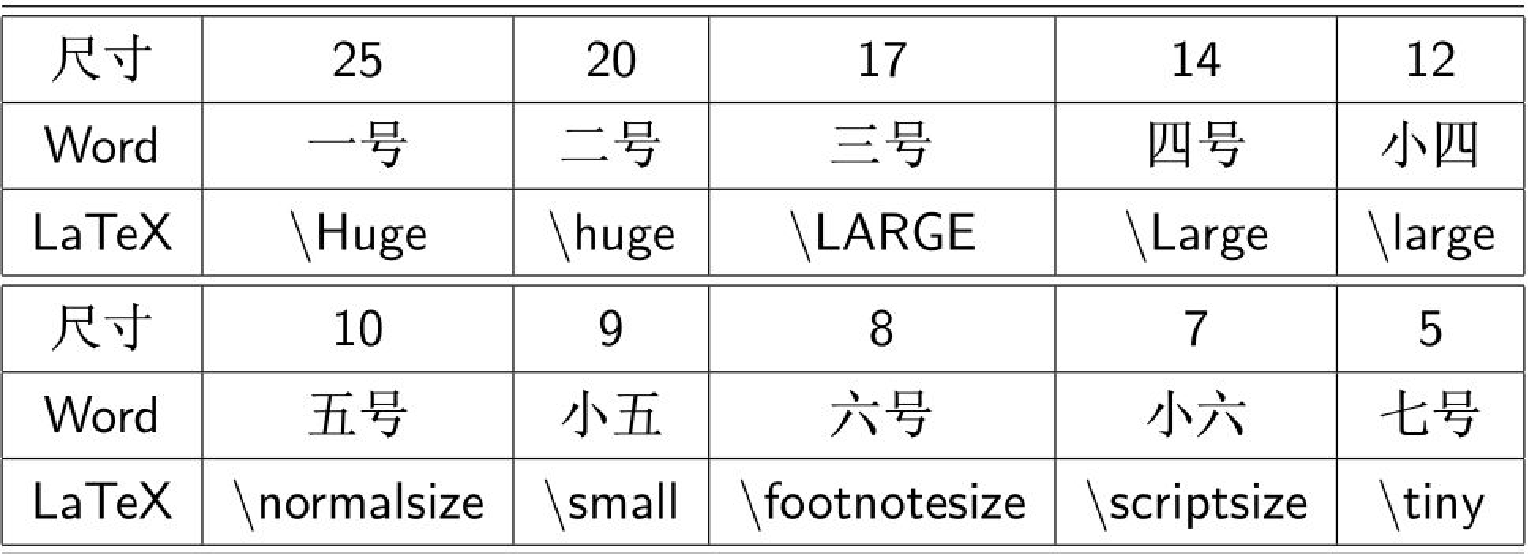
\includegraphics[scale=0.3]{latex_fontsize.pdf}
    \end{figure}

    用法参考:\\
    这是\{$\backslash$normalsize 普通字体\},这是\{$\backslash$small 小字体\}
  }

  \frame
  {
    \frametitle{特殊符号示例}
    \begin{figure}
    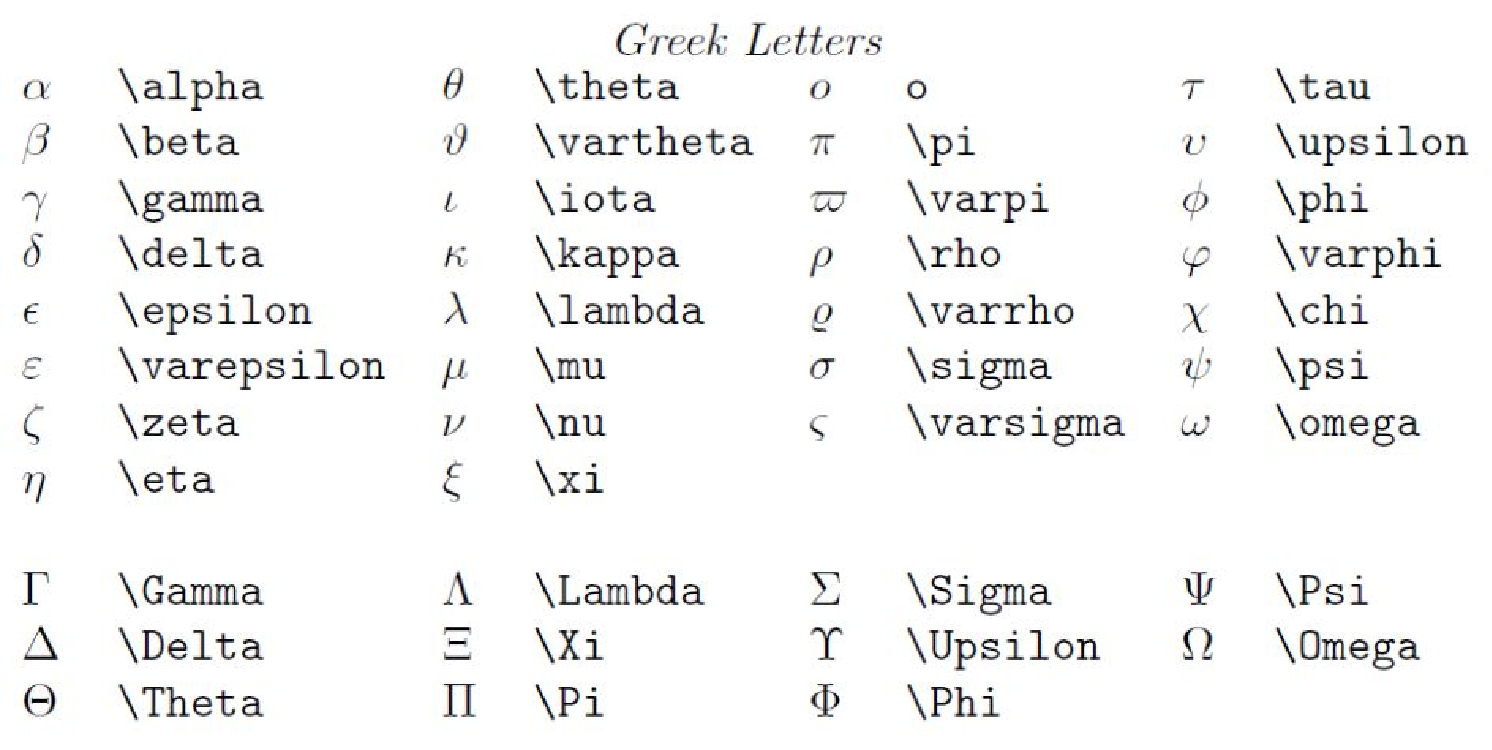
\includegraphics[scale=0.3]{latex_symb.pdf}
    \end{figure}

    大部分符号需要包括amsmath宏包:\\ $\backslash$usepackage\{amsmath\}
  }

  \frame
  {
    \frametitle{章节环境}
    \begin{itemize}
    \item 篇(part)
    \item 章(chapter)
    \item 节(section)
    \item 小节(subsection, subsubsection)
    \item 段(paragraph, subparagraph)
    \end{itemize}

    用法示例:\\
    $\backslash$section\{简介\}
  }

  \subsection{数学公式排版}
  \frame
  {
    \frametitle{\subsecname}
    \begin{itemize}
    \item 行中数学公式\\
    $\backslash$begin\{math\}数学公式$\backslash$end\{math\}
      \begin{itemize}
      \item 简式1:$\backslash$(数学公式$\backslash$)
      \item 简式2:\$ 数学公式 \$
      \end{itemize}
    \item 行间数学公式\\
    $\backslash$begin\{equation\}数学公式$\backslash$end\{equation\}
      \begin{itemize}
      \item 简式1:$\backslash$[数学公式$\backslash$]
      \item 简式2:\$\$ 数学公式 \$\$
      \end{itemize}
    \end{itemize}
  }

  \frame
  {
    \frametitle{\subsecname}

    上帝创造了欧拉公式:$e^{i\pi}+1=0$。

    \begin{equation*}
    \frac{1}{\sqrt{2\pi}}\int_{-\infty}e^{-{x^2} \over 2}\,dx = 1
    \end{equation*}

    \begin{equation*}
    \left[\begin{array}{cccc}
    1 &  6  & 9 \\
    7 &  90  & f(x) \\
    9 &  \psi(x)  &g(x)
    \end{array} \right]
    \end{equation*}
  }

  \subsection{BibTeX 文献管理}
  \frame
  {
    \frametitle{\subsecname}
    BibTeX是一种格式和一个程序,用于协调\LaTeX 的参考文献。它使用数据库的方式来管理参考文献,数据库后缀名.bib。\\
    数据库中存放参考文献条目,例如:

    \begin{figure}
    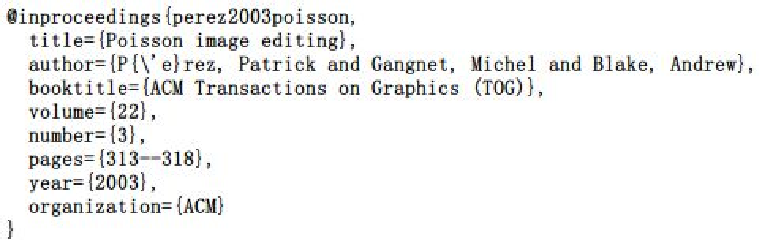
\includegraphics[scale=0.6]{bibtex_example.pdf}
    \end{figure}
  }

  \frame
  {
    \frametitle{\subsecname}
    在你的整个研究生涯,可以只维护一个.bib文件,它就是一个数据库,每个参考文献是一个记录,由一个唯一的ID描述。当你需要引用相关文献时,使用$\backslash$cite\{\}即可引用你的文献数据库中的论文。
  }

  \subsection{制作演讲稿(slide)}

  \frame
  {
    \frametitle{\LaTeX 制作slide的实现途径}
    \begin{itemize}
    \item beamer
    \item foiltex
    \item prosper
    \item pdfscreen
    \end{itemize}
  }

  \frame
  {
    \frametitle{关于Beamer}
    Beamer是\LaTeX 上用来制作slide的一个文档类,它的特点是同标准\LaTeX 结合度高,不需要其他后处理程序:
    \begin{enumerate}
    \item 使用part,section,subsection等命令组织逻辑结构
    \item 使用frame命令组织内容
    \item 使用theme,template,logo改变缺省风格
    \item 使用overlay选项控制临时效果
    \item 通过文档类选项控制输出格式等
    \end{enumerate}
  }

  \frame
  {
    \frametitle{总结}
    \begin{itemize}
    \item 使用\LaTeX 撰写高质量的科技类文档
    \item \LaTeX 是科研界的标准
    \item \LaTeX 专注于文章逻辑内容,不适合大量图文混排文档
    \item 使用BibTeX管理文献
    \item 使用Beamer制作风格简洁,内容清晰的演示文稿
    \end{itemize}
  }

  \frame
  {
    \frametitle{关于\LaTeX 学习的建议}
    \begin{itemize}
    \item 在使用中学习,多查文档
    \item 记录使用中出现的问题,如编译错误的解决过程,某个具体问题的解决方法
    \item 多积累模板,打造自己的模板库
    \end{itemize}
  }

  \frame
  {
    \frametitle{完}
    \vspace{2cm}
    {\huge 谢谢!}
    \epigraph{对于出卖其灵魂的人来说,\LaTeX 不能很好的工作...}{lshort}
  }
  \end{document}
